\chapter{Dasar Pemrograman Python}
\section{Pendahuluan}
Bahasa pemrograman Python memiliki 4 sifat dasar berikut\footnote{\url{https://www.tutorialspoint.com/python/index.htm}}.
\begin{enumerate}
  \item \textit{Interpreter}. Python diproses oleh \textit{interpreter}, sehingga tidak perlu dikompilasi untuk menjalankannya. Hal ini seperti dijumpai pada bahasa pemrograman PHP yang sangat populer itu.
  \item Interaktif. Anda dapat berinteraksi denga Python dengan memberikannya perintah satu per satu melalui Python \texttt{shell}. Setiap perintah yang diberikan langsung akan direspon. Selain itu, Python bersifat \textit{self explained}. Jika ada fungsi dari suatu obyek yang tidak kita ketahui, kita bisa mempelajarinya langsung dari dokumentasi di Python \texttt{shell}.
  \item Berorientasi obyek. Ada semacam slogan bahwa '''\textit{Everything is object in Python}'''. Seperti telah dipahami melalu kuliah Rekayasa Perangkat Lunak, orientasi obyek menyebabkan variabel dan fungsi (sering disebut sebagai \textit{state} dan \textit{behavior}) terkemas dalam sebuah obyek, sehingga memudahkan pengelolaan variabel. Fungsi yang melekat pada sebuah obyek juga dapat diturunkan dari satu obyek ke obyek lain sehingga tidak perlu dideklarasi ulang. Namun, fitur orientasi obyek ini pemberlakuannya bagi pemrogram tidak seketat seperti yang dilakukan di \texttt{Java}. Jika \texttt{Java} mengharuskan pemrogram mendeklarasikan kelas untuk membuat program yang bahkan sangat sederhana, makan Python tidak mengharuskannya.
  \item Bahasa pemrograman untuk pemula. Hal ini disebabkan karena Python sangat sederhana, tidak memerlukan banyak deklarasi yang seringkali menyulitkan, bahkan menakutkan bagi pemula. Selain itu, Python juga mendukung pengembangan aplikasi untuk banyak \textit{platform}, dari aplikasi \textit{embedded} hingga \textit{web} dan \textit{mobile}. 
\end{enumerate}

Untuk sifat dasar pertama dan kedua, dapat dilihat ilustrasinya di \figurename~\ref{fig:interpreter}. Dalam \figurename~\ref{fig:interpreter}, Python \texttt{shell} dipanggil dengan perintah \texttt{python3}. Hal tersebut disebabkan karena Ubuntu (yang sedang digunakan adalah Ubuntu 18.04) secara \textit{default} menyertakan Python versi 2.x. Sedangkan untuk Python versi 3.x harus dijalankan dengan perintah \texttt{python3}. Di \figurename~\ref{fig:interpreter} terlihat bahwa ada dua perintah yang diberikan secara berurutan. Tetapi, Python akan meresponnya satu per satu. Sedangkan untuk keluar dari Python \texttt{shell}, berikan perintah \texttt{exit()}.

\begin{figure}[h!]
  \begin{center}
    \includegraphics[scale=.5]{pics/interpreter.png}
    \caption{Python \texttt{shell} sedang menerima perintah}
    \label{fig:interpreter}
  \end{center}
\end{figure}

Untuk sifat dasar ketiga dapat diilustrasikan melalui \figurename~\ref{fig:obyek}. Kita dapat mengetahui jenis obyek dari variabel \texttt{a} dengan fungsi \texttt{type(a)}. Sedangkan untuk melihat fungsi dan variabel apa saja yang terkandung pada variabel \texttt{a}, kita dapat menggunakan fungsi \texttt{dir(a)}. Tetapi, meskipun semuanya di dalam Python adalah obyek, penggunaan Python tidak mengharuskan kita mendeklarasi kelas secara eksplisit. Dengan menuliskan perintah \texttt{a=3}, Python tahu bahwa obyek \texttt{a} adalah obyek dari kelas \texttt{integer}. Bahkan, di \figurename~\ref{fig:interpreter}, operasi aritmatika dapat dilakukan tanpa mendeklrasi variabel.

\begin{figure}[h!]
  \begin{center}
    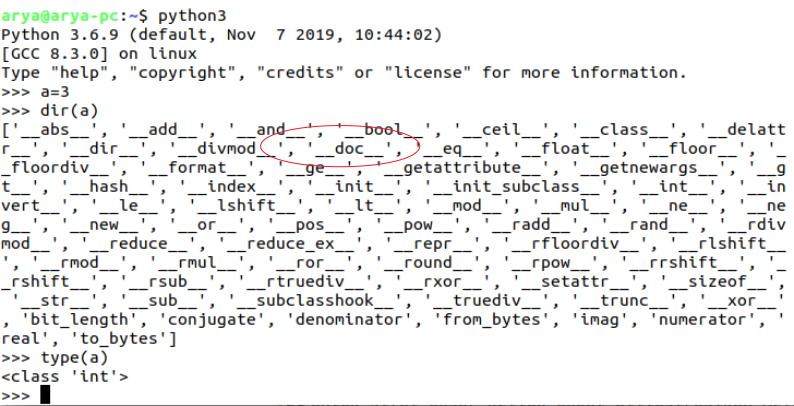
\includegraphics[scale=.5]{pics/interpreter2a.png}
    \caption{Variabel \texttt{a} sebagai obyek}
    \label{fig:obyek}
  \end{center}
\end{figure}

Di \figurename~\ref{fig:obyek} terlihat ada entitas yang diawali dan/atau diakhir dengan karakter dua \textit{underscore} ('\_\_') atau sering disebut sebagi \textit{dunder}\footnote{\url{https://dbader.org/blog/meaning-of-underscores-in-python}} (\textit{double undescore}) oleh komunitas pemrogram Python. Hal tersebut merupakan bagian dari PEP (\textit{Python Enhancement Proposals}) ke-8 tentang \textit{Style Guide for Python Code}\footnote{\url{https://www.python.org/dev/peps/pep-0008/}}.

Di \figurename~\ref{fig:obyek} juga terlihat bahwa obyek \texttt{a} memiliki fungsi \texttt{\_\_doc\_\_}. Fungsi inilah yang akan memberikan penjelasan singkat kepada kita tentang obyek yang sedang menjadi perhatian. Untuk menggunakannya, jalankan perintah \texttt{a.\_\_doc\_\_} seperti ditunjukkan \figurename~\ref{fig:doc}. Dengan \texttt{a} adalah nama variabel untuk obyek yang sedang menjadi perhatian.

\begin{figure}[h!]
  \begin{center}
    \includegraphics[scale=.5]{pics/interpreter3.png}
    \caption{Menampilkan dokumentasi obyek \texttt{integer a}}
    \label{fig:doc}
  \end{center}
\end{figure}

Format dokumentasi seperti yang ditunjukkan pada \figurename~\ref{fig:doc} sulit untuk dipahami. Pendekatan lain untuk mempelajari dokumentasi sebuah pustaka adalah dengan menggunakan fungsi \texttt{help}. Untuk kasus seperti \figurename~\ref{fig:doc}, perintah yang dijalankan adalah \texttt{help(a)} (\textbf{BUKAN} \texttt{a.\_\_doc\_\_}). Hasilnya ditunjukkan pada \figurename~\ref{fig:doc2}. Untuk keluar dari modus dokumentasi tersebut, pengguna tinggal memberi perintah \texttt{q} setelah tanda titik dua (\figurename~\ref{fig:doc2}). Sedangkan untuk melihat isi dokumentasi selanjutnya pengguna dapat menggunkana tombol spasi di papan ketik.

\begin{figure}
  \begin{center}
    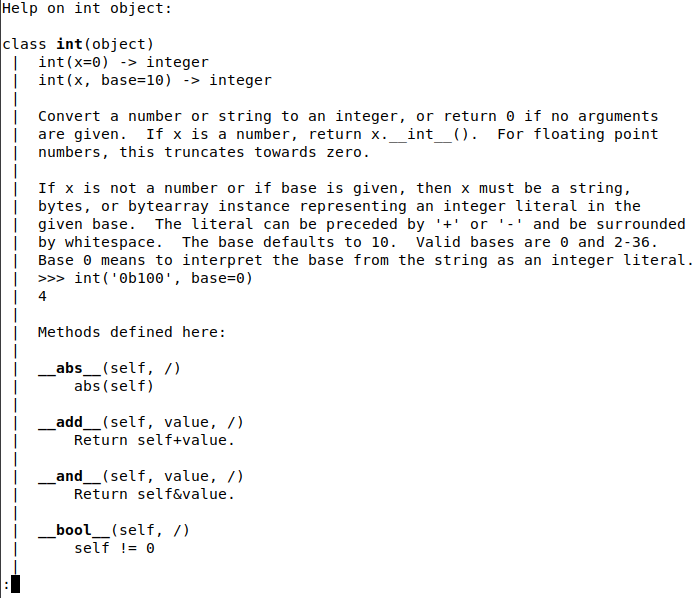
\includegraphics[scale=.5]{pics/interpreter4.png}
    \caption{Menampilkan dokumentasi obyek \texttt{integer a} menggunakan fungsi \texttt{help}}
    \label{fig:doc2}
  \end{center}
\end{figure}
